% =============================================================================
%  Soutenance — Dynamic Monitoring of Radiological Pollution through Deep Learning
%  Beamer slides mirroring the structure of the final report (../sections/*.tex).
%  Build (from this folder):  pdflatex slides   (run twice for the outline TOC)
%  Figures are reused from ../figures/ (the report's figure set).
% =============================================================================
\documentclass[11pt, aspectratio=169]{beamer}

\usetheme{metropolis}
\metroset{progressbar=frametitle, numbering=fraction, block=fill, sectionpage=none}

\usepackage{appendixnumberbeamer}     % keep main numbering clean across the appendix
\usepackage[T1]{fontenc}
\usepackage[utf8]{inputenc}
\usepackage[english]{babel}
\usepackage{amsmath, amssymb, mathtools}
\usepackage{bm}
\usepackage{booktabs}
\usepackage{graphicx}
\usepackage{xcolor}
\usepackage{tikz}
\usetikzlibrary{positioning, arrows.meta, calc}

\graphicspath{{../figures/}{figures/}}

% ── Palette (a calm CentraleSupélec-style blue) ──────────────────────────────
\definecolor{csblue}{HTML}{1F4E79}
\definecolor{csaccent}{HTML}{2E75B6}
\setbeamercolor{frametitle}{bg=csblue}
\setbeamercolor{progress bar}{fg=csaccent}
\setbeamercolor{alerted text}{fg=csaccent}
\setbeamertemplate{frametitle continuation}{}

% ── Math macros (identical to the report's preamble.tex) ─────────────────────
\newcommand{\R}{\mathbb{R}}
\newcommand{\softmax}{\operatorname{softmax}}
\newcommand{\ReLU}{\operatorname{ReLU}}
\newcommand{\Conv}{\operatorname{Conv1D}}
\newcommand{\BN}{\operatorname{BN}}
\newcommand{\GN}{\operatorname{GN}}
\newcommand{\Attn}{\operatorname{Attention}}
\newcommand{\dCNN}{1D-CNN}
\newcommand{\dResNet}{ResNet 1D}
\newcommand{\dAttn}{CNN+Attention}

% slightly tighter itemize for dense slides
\setlength{\leftmargini}{1.1em}
\setbeamertemplate{itemize items}[circle]

% ── Title metadata ───────────────────────────────────────────────────────────
\title{Dynamic Monitoring of Radiological Pollution\\ through Deep Learning}
\subtitle{Classifying anomaly shapes in noisy gamma-dose time series}
\author{Pedro De Bem \\[0.2em] {\footnotesize\itshape [co-authors --- to be completed]}}
\institute{CentraleSupélec --- Pôle Projet Data Science\\
           Supervised by Elisabeth Lahalle (L2S)}
\date{Project defense --- June 2026}

\begin{document}

% ── 1. Title ─────────────────────────────────────────────────────────────────
{\setbeamertemplate{footline}{}
\begin{frame}[plain]
  \maketitle
\end{frame}}

% ── 2. Context (short introduction, before the plan) ─────────────────────────
\begin{frame}{Context: monitoring radiological pollution}
  \begin{columns}[T]
    \begin{column}{0.6\linewidth}
      \begin{itemize}
        \item Environmental beacons count the \alert{gamma photons} reaching a
              scintillation detector, once per minute $\rightarrow$ a
              \alert{gamma-dose} time series.
        \item It reflects the natural radioactive background, modulated by
              weather and --- rarely --- by a radiological \alert{event}
              (passing source, leak, plume).
        \item Operational goal: \alert{detect and identify} such events as
              early as possible, from the \emph{shape} they leave in the signal.
      \end{itemize}
      \vspace{0.4em}
      {\footnotesize \textbf{Why it is hard:}}
      \begin{itemize}\footnotesize
        \item per-sample noise $\approx$ the size of weak events;
        \item the baseline drifts slowly with weather $\Rightarrow$ no fixed
              threshold works;
        \item different phenomena leave different signatures $\Rightarrow$ one
              must \emph{classify the shape}, not merely detect.
      \end{itemize}
    \end{column}
    \begin{column}{0.4\linewidth}
      \centering
      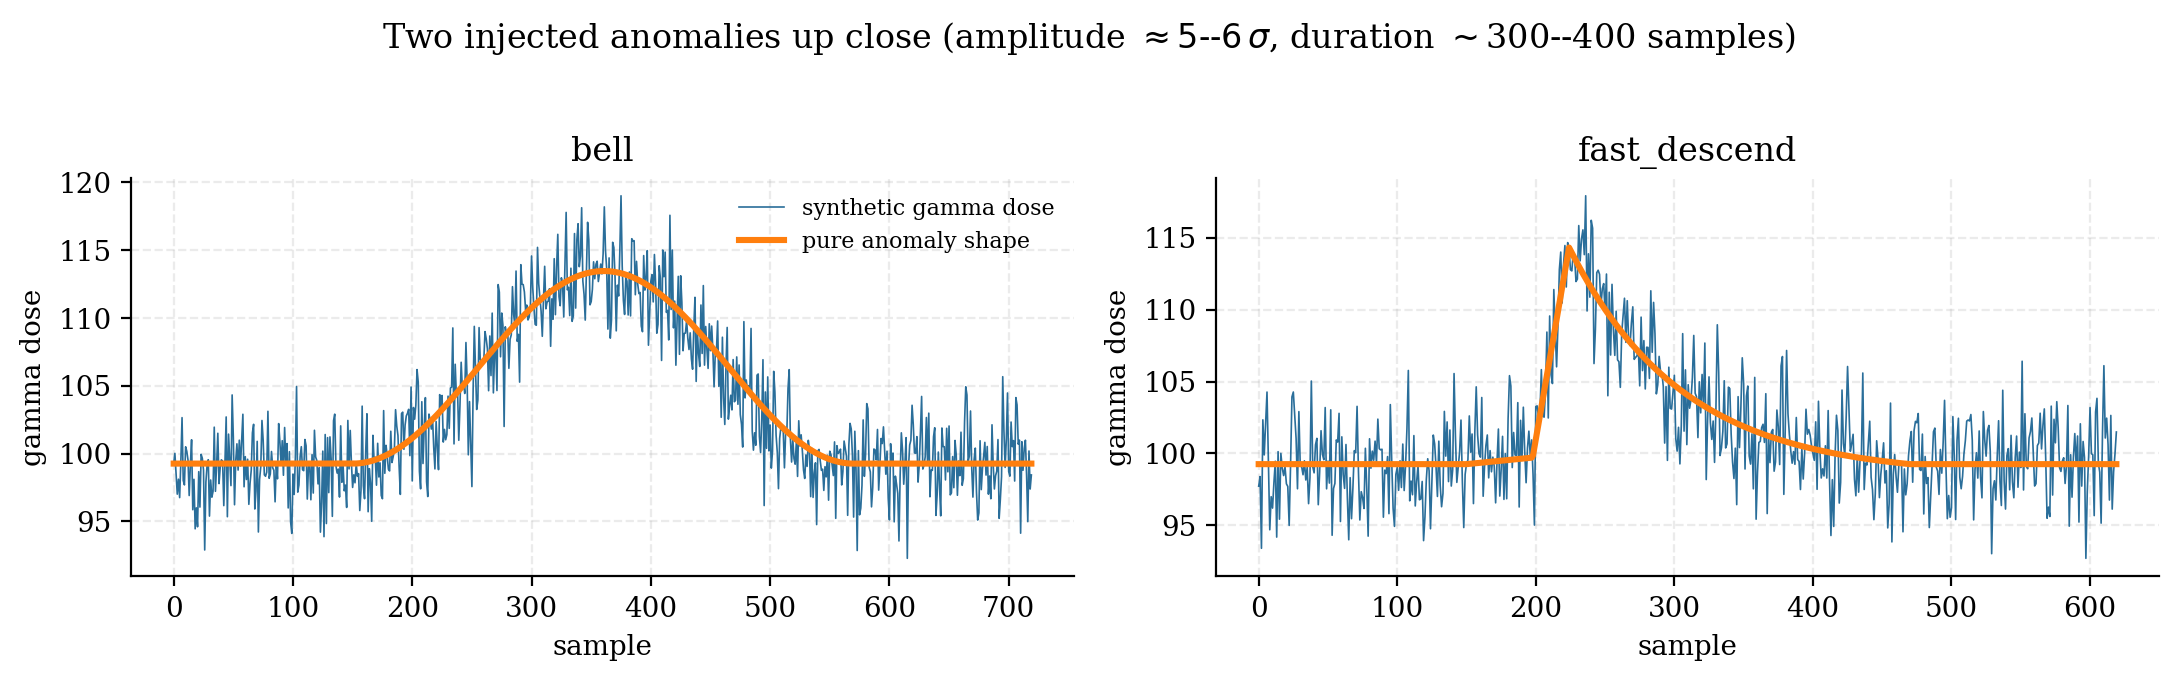
\includegraphics[width=\linewidth]{anomaly_snapshots}\\[0.3em]
      {\scriptsize Two events in the synthetic signal: a smooth \texttt{bell}
       (left) and an asymmetric \texttt{fast\_descend} (right).}
    \end{column}
  \end{columns}
\end{frame}

% ── 3. Outline (the plan, announced after the short intro) ───────────────────
\begin{frame}{Outline}
  \tableofcontents
\end{frame}

% =============================================================================
\section{Problem and objectives}
% =============================================================================

\begin{frame}{Problem: windowed multi-class classification}
  Treat event identification as \alert{supervised classification of a univariate
  signal}.
  \begin{itemize}
    \item Gamma-dose series $x = (x_1,\dots,x_N) \in \R^{N}$; $x_t$ = value at
          minute $t$, $N$ samples.
    \item Each instant belongs to one of $K$ classes: label $0$ =
          \texttt{Normal Background}, and $K-1$ anomaly morphologies. Here
          $K = 7$.
    \item A class is defined by the local \emph{shape}, not by $x_t$
          $\Rightarrow$ classify \alert{fixed-length windows}, not samples.
  \end{itemize}
  \begin{block}{Windowing and classifier}
    \[
      \mathbf{x}^{(t)} = (x_{t-W+1},\dots,x_t) \in \R^{W},
      \qquad
      \hat{p}^{(t)} = \softmax\!\big(f_\theta(\mathbf{x}^{(t)})\big) \in \Delta^{K-1}.
    \]
    {\footnotesize
     $W$ = window length ($W=512 \approx 8.5$\,h); $f_\theta:\R^{W}\!\to\R^{K}$ =
     network with parameters $\theta$ (outputs class logits);
     $\Delta^{K-1}$ = probability simplex (entries $\ge 0$, summing to $1$).
     Each window gets one label $y^{(t)}\in\{0,\dots,K-1\}$ (coverage rule, later).}
  \end{block}
\end{frame}

\begin{frame}{Objectives and approach}
  \textbf{Training objective} --- class-weighted cross-entropy:
  \[
    \mathcal{L}(\theta) = -\frac{1}{|\mathcal{D}|}
        \sum_{(\mathbf{x},y)\in\mathcal{D}} w_y \,\log
        \softmax\!\big(f_\theta(\mathbf{x})\big)_y,
    \qquad
    w_c = \frac{|\mathcal{D}|}{K\,n_c}.
  \]
  {\footnotesize $\mathcal{D}$ = labelled training windows, $|\mathcal{D}|$ its
   size; $n_c$ = number of windows of class $c$; the weight $w_c$ compensates
   class imbalance.}
  \vspace{0.3em}
  \begin{itemize}
    \item \textbf{Evaluation objective:} window accuracy over-counts background
          $\Rightarrow$ report an \alert{event-level macro $F_1$}: window
          probabilities are accumulated into a per-sample trace, contiguous
          non-background runs form predicted events, each is matched to a true
          event (precision/recall, $F_1$ averaged over anomaly classes).
    \item \textbf{Why deep learning:} a classical baseline-removal $+$
          matched-filter bank scales poorly (time-warp, noise, every new
          morphology $\Rightarrow$ redesign); CNN/attention \emph{learn} shape
          features.
    \item \textbf{What we validate:} no labelled real events exist $\Rightarrow$
          we train \& evaluate on a \alert{calibrated synthetic benchmark};
          real-data evaluation is deliberately out of scope.
  \end{itemize}
\end{frame}

% =============================================================================
\section{Related work and positioning}
% =============================================================================

\begin{frame}{Related work --- what we build on}
  \footnotesize
  \begin{block}{Deep learning for time-series classification (TSC)}
    Shift from distance-based methods (1-NN $+$ DTW) to deep nets. Ismail Fawaz
    et al.\ (2019) and Wang et al.\ (2017) find fully-convolutional and 1D
    residual networks the strongest general baselines $\rightarrow$ motivates our
    \emph{conv baseline} and \emph{residual} variant. TCNs (Bai et al.\ 2018):
    convolutions match/beat RNNs, more cheaply.
  \end{block}
  \begin{block}{Convolutional / residual networks and normalisation}
    Weight-shared local filters (LeCun et al.\ 1998) give translation
    equivariance and length-independent parameters; residual connections (He et
    al.\ 2016) make depth trainable. BatchNorm (Ioffe \& Szegedy 2015) vs
    GroupNorm (Wu \& He 2018, identical at train/inference --- exploited for a
    drifting amplitude).
  \end{block}
  \begin{block}{Attention, hybrids, anomaly detection \& explainability}
    Self-attention / Transformers (Vaswani et al.\ 2017), LayerNorm (Ba et al.\
    2016) and the \texttt{[CLS]} token (Devlin et al.\ 2019). CNN--Transformer
    hybrid for noisy physiological signals (Hu \& Chen 2022, in the brief). We
    borrow event-level evaluation from the anomaly-detection survey
    (Bl\'azquez-Garc\'ia et al.\ 2021); explainability via Grad-CAM (Selvaraju
    et al.\ 2017).
  \end{block}
\end{frame}

\begin{frame}{Positioning and contribution}
  \begin{itemize}
    \item We \alert{adopt established architectures} rather than proposing a new
          one: a convolutional baseline, a residual network (He 2016; Wang 2017),
          and a CNN--Transformer hybrid (Vaswani 2017; Hu 2022).
  \end{itemize}
  \begin{block}{The contribution is methodological and applicative}
    \begin{enumerate}
      \item a \alert{simplified yet statistically calibrated} synthetic
            generator for noisy gamma-dose signals with controllable anomaly
            morphologies;
      \item a controlled, \alert{like-for-like comparison} of the three
            architectures along the three axes named in the project brief ---
            \emph{classification performance}, \emph{computational cost}, and
            \emph{robustness to distribution shift}.
    \end{enumerate}
  \end{block}
  \begin{itemize}
    \item To our knowledge this combination has not been reported for
          radiological-beacon anomaly classification.
  \end{itemize}
\end{frame}

% =============================================================================
\section{Signal model and synthetic data}
% =============================================================================

\begin{frame}{Real data: a brief characterisation}
  \begin{columns}[T]
    \begin{column}{0.46\linewidth}
      \begin{itemize}
        \item Four months of 2015 gamma-dose recordings (Feb, Apr, Jun, Oct),
              $\approx 40{,}000$ samples each, $1$ / minute.
        \item Two components:
              \begin{itemize}\footnotesize
                \item a slowly drifting \alert{baseline} near $99$ counts;
                \item a zero-mean \alert{high-frequency} fluctuation,
                      $\sigma \approx 2.3$--$2.7$ counts.
              \end{itemize}
        \item These few numbers are \emph{all} we take from the real data ---
              they calibrate the synthetic generator.
      \end{itemize}
    \end{column}
    \begin{column}{0.54\linewidth}
      \centering
      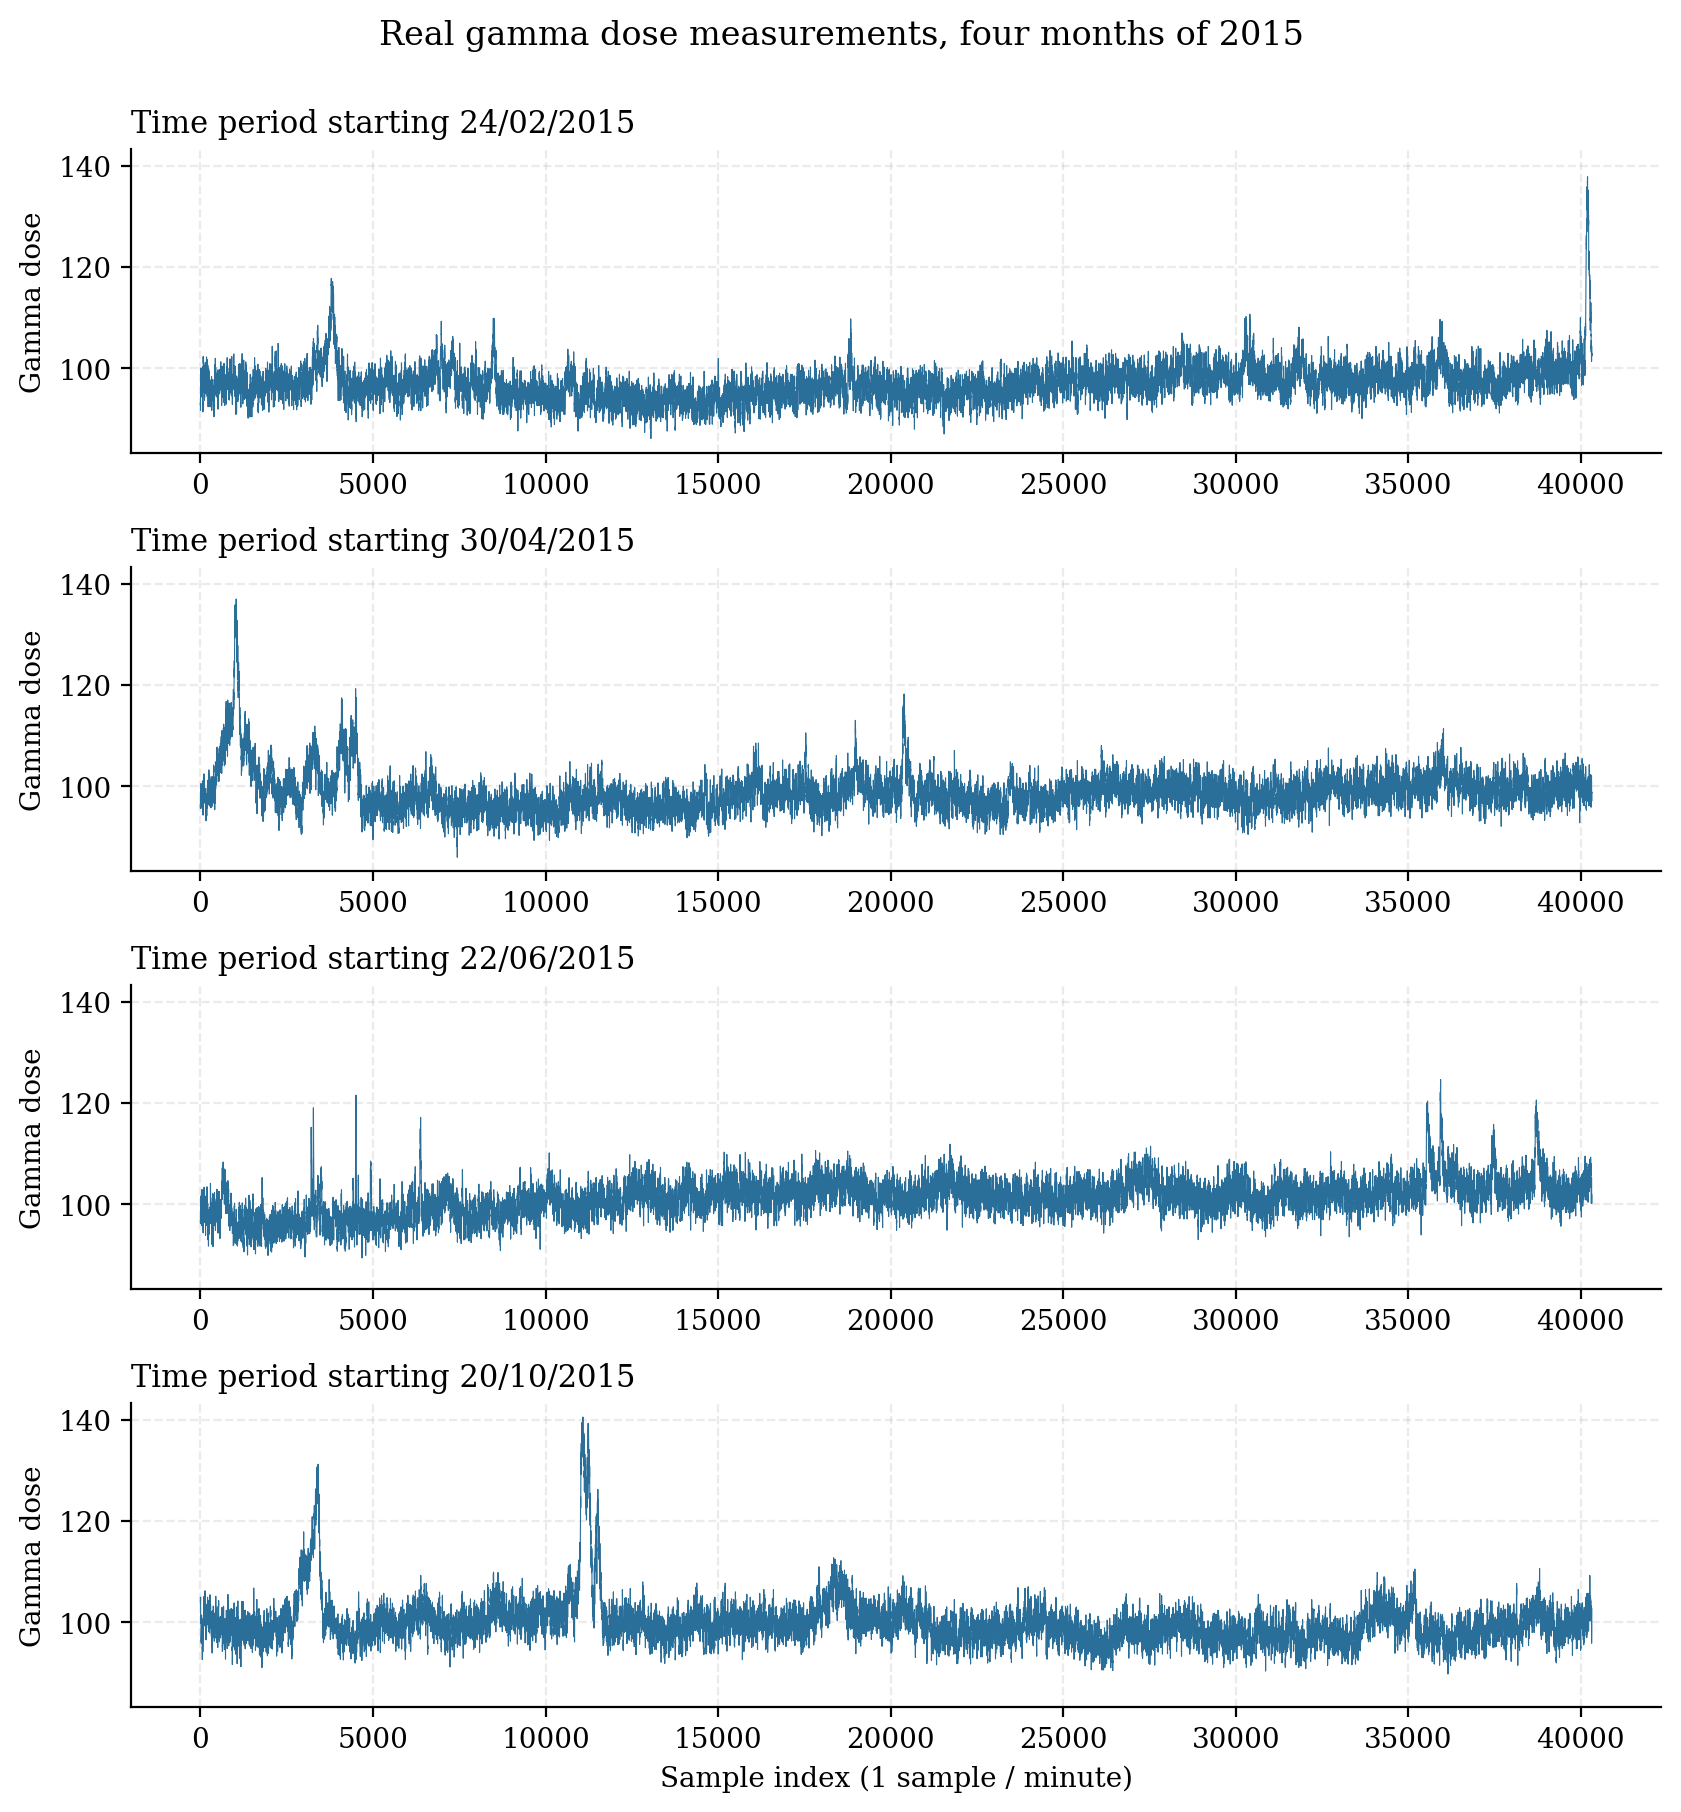
\includegraphics[height=0.74\textheight]{real_data_overview}
    \end{column}
  \end{columns}
\end{frame}

\begin{frame}{Synthetic background model}
  White Gaussian high-frequency noise on a slowly drifting
  \alert{Ornstein--Uhlenbeck} (mean-reverting) baseline:
  \[
    x_t = b_t + \eta_t,\quad \eta_t \overset{\text{iid}}{\sim}\mathcal{N}(0,\sigma^2),
    \qquad
    b_{t+1} = b_t + \theta\,(\mu - b_t) + \xi_t,\quad
    \xi_t \overset{\text{iid}}{\sim}\mathcal{N}(0,\sigma_{\mathrm{OU}}^2).
  \]
  {\footnotesize $b_t$ = baseline; $\eta_t$ = high-frequency sensor noise;
   $\mu$ = long-run mean level; $\theta$ = mean-reversion rate; $\sigma$ = HF
   noise std; $\sigma_{\mathrm{OU}}$ = baseline-innovation std.}
  \vspace{0.5em}
  \begin{itemize}
    \item Calibrated to the four real months:
          $\mu = 99.26$, $\sigma = 2.53$, $\theta = 4\cdot 10^{-6}$,
          $\sigma_{\mathrm{OU}} = 0.0373$.
    \item Tiny $\theta$ $\Rightarrow$ the baseline drifts over hundreds of
          thousands of samples, far slower than the $W=512$ window.
    \item \alert{Deliberately crude}: it captures the marginal noise level and
          slow drift, but treats the HF noise as time-independent --- the main
          simplification we accept (see Perspectives).
  \end{itemize}
\end{frame}

\begin{frame}{Anomaly morphologies}
  \begin{columns}[T]
    \begin{column}{0.46\linewidth}
      \begin{itemize}
        \item Six morphologies $\rightarrow$ $K=7$ classes with the background:
              \texttt{bell}, \texttt{bell\_sq}, \texttt{fast\_ascend},
              \texttt{fast\_descend}, \texttt{M}, \texttt{square}.
        \item Stored as \alert{keypoints} joined by linear / exponential /
              half-cosine segments.
        \item Every injected anomaly is \alert{randomly deformed}: keypoints
              jittered by a Gaussian of std $\nu$ (the deformation level),
              shape-preserving constraints, then rescaled.
      \end{itemize}
      \vspace{0.2em}
      \begin{block}{Sampling ranges}
        \footnotesize
        amplitude $\in \sigma\cdot[2.5,\,7.6]$ (in noise-$\sigma$, i.e.\ SNR
        units), \;duration $\in [200,800]$ samples, \;$\nu \in [0.02,0.10]$.
      \end{block}
    \end{column}
    \begin{column}{0.54\linewidth}
      \centering
      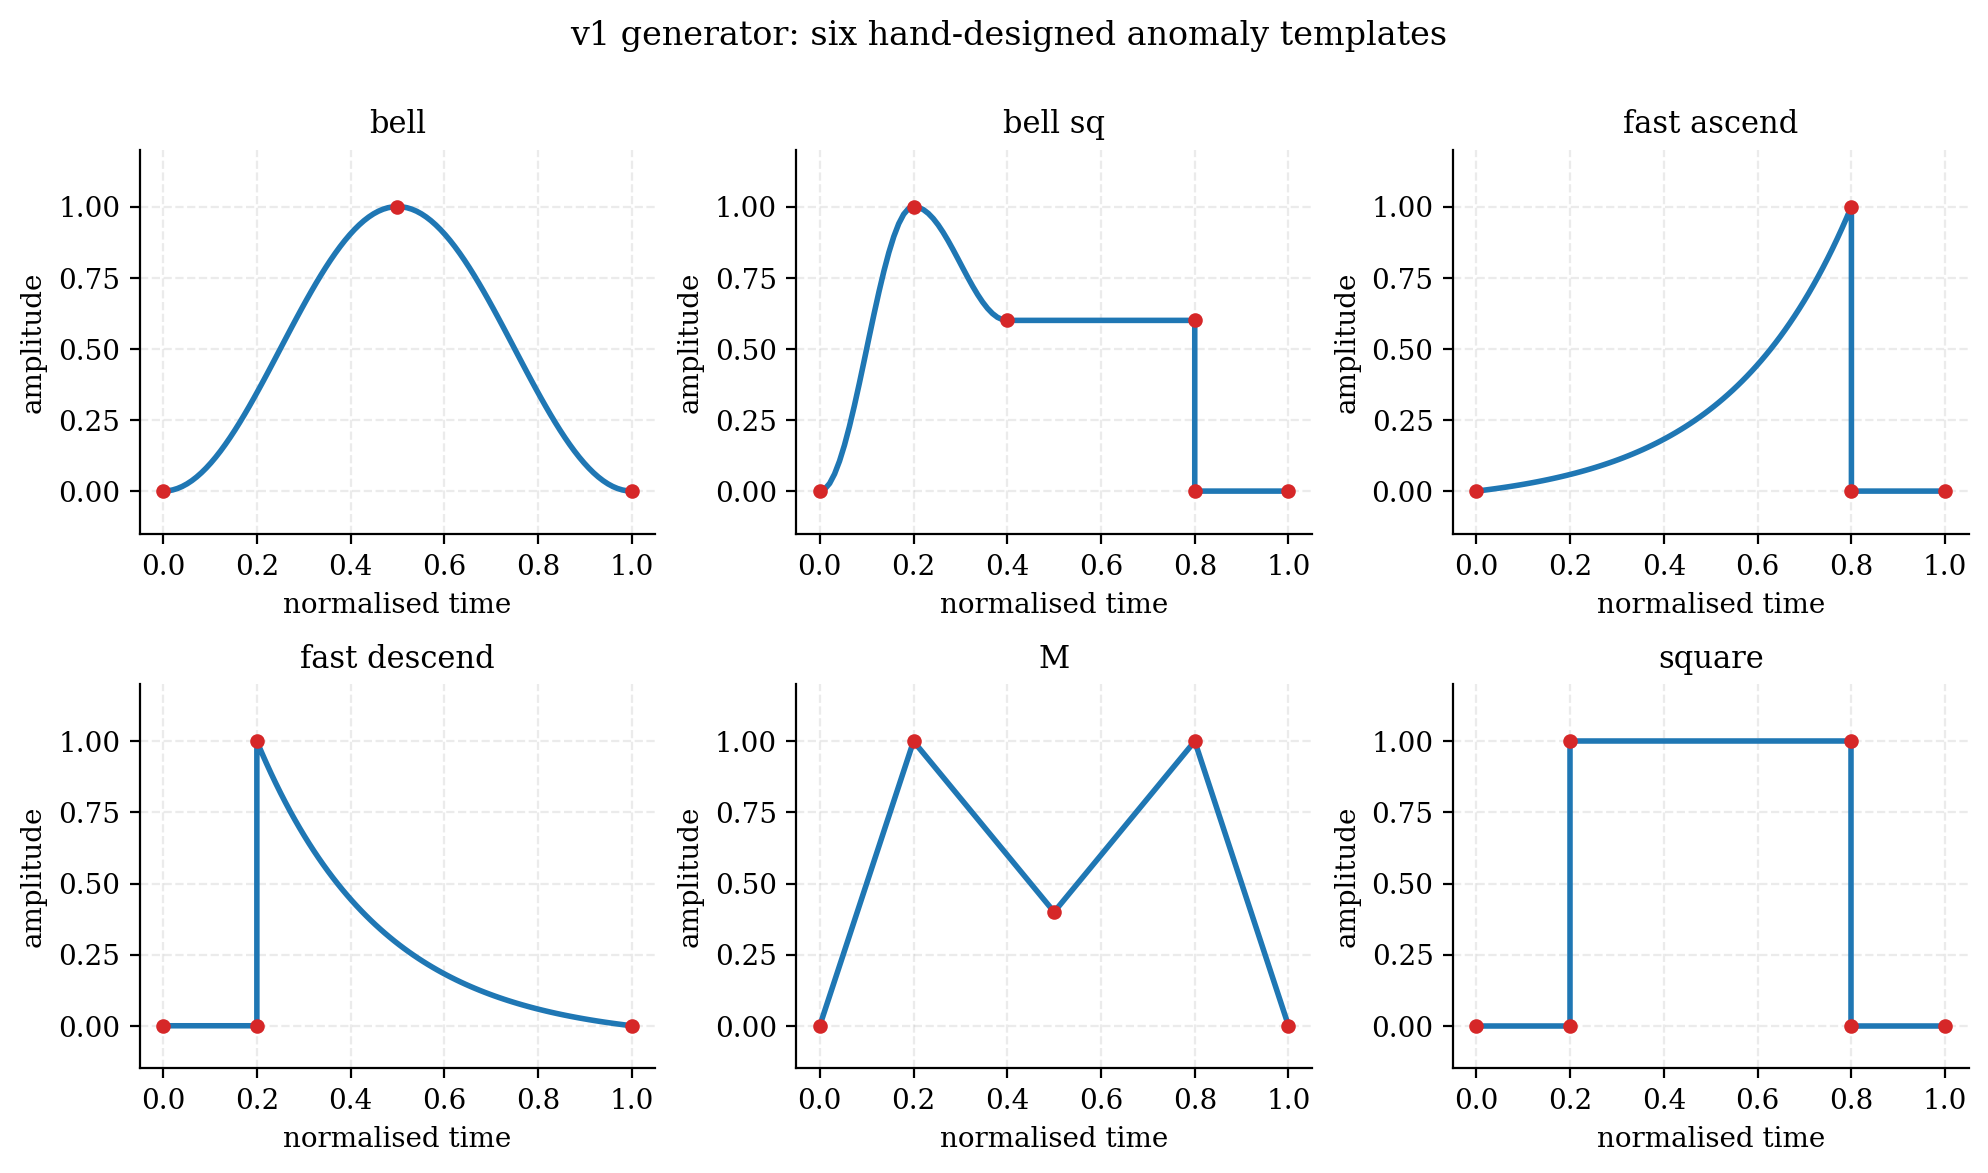
\includegraphics[width=\linewidth]{v1_anomaly_templates}
    \end{column}
  \end{columns}
\end{frame}

\begin{frame}{The synthetic dataset}
  \centering
  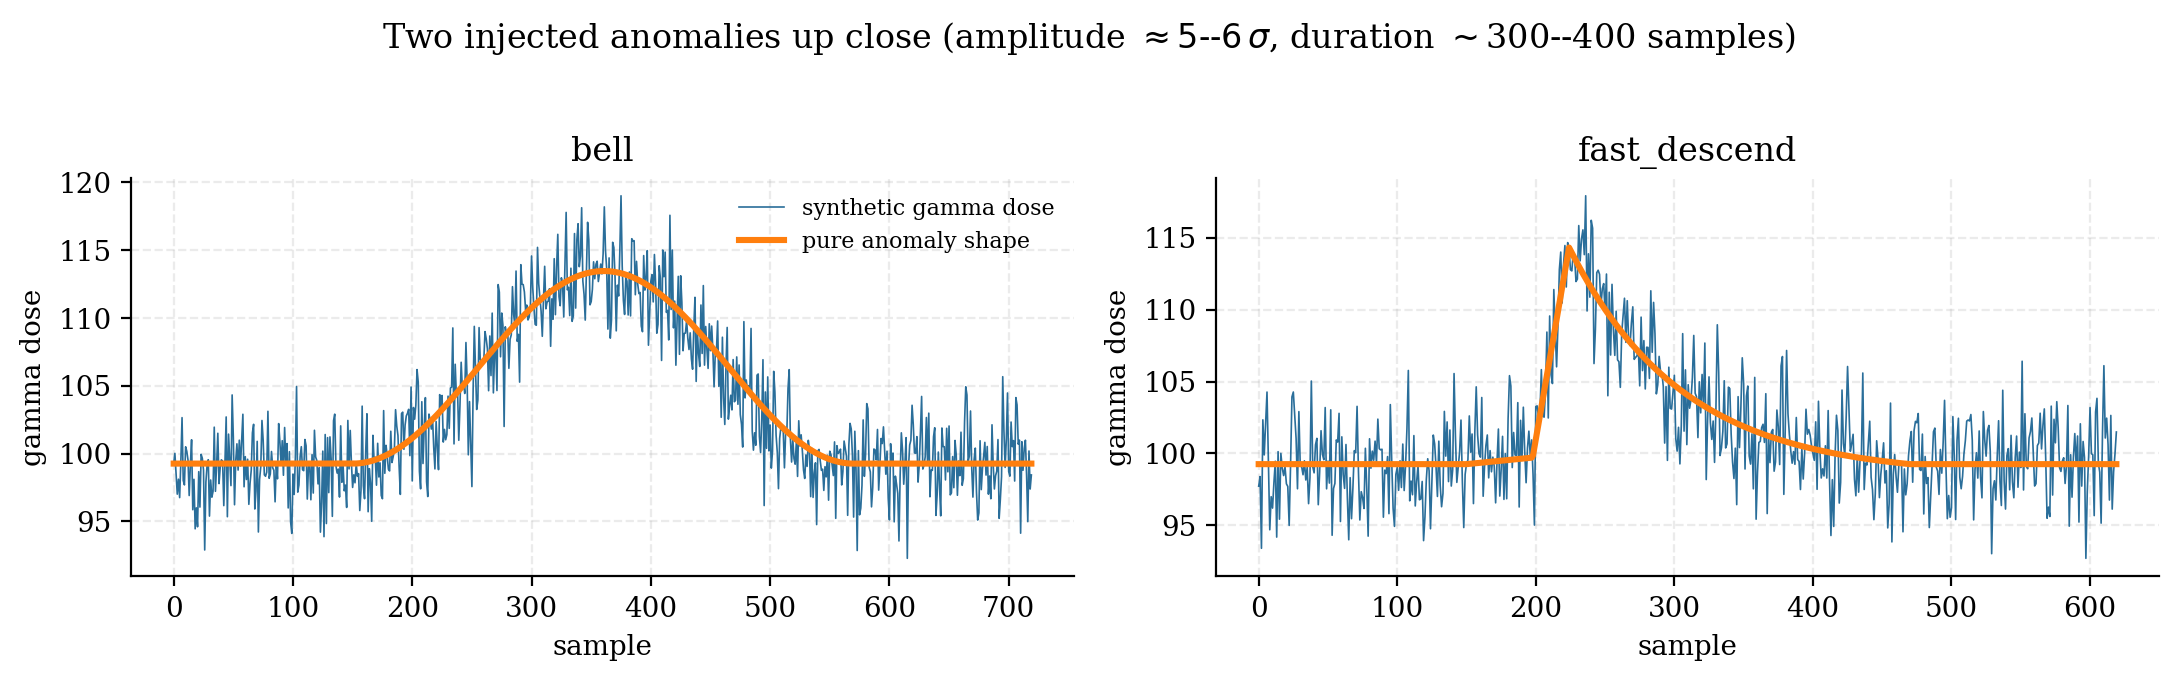
\includegraphics[width=0.96\linewidth]{anomaly_snapshots}
  \begin{itemize}
    \item Generator combines the background with injected, deformed anomalies
          (blue = generated dose, orange = clean shape before noise).
    \item Dataset used throughout: $N = 10^{7}$ samples, $5{,}000$--$8{,}000$
          anomalies ($\sim 6$--$8$ events / $10$k samples).
    \item \alert{Dense injection} = abundant, balanced examples of every
          morphology --- at the cost of a background prior far denser than a
          real beacon's (a gap we revisit).
  \end{itemize}
\end{frame}

% =============================================================================
\section{Methods: architectures and training}
% =============================================================================

\begin{frame}{Input pipeline: windowing, labelling, normalisation}
  \centering
  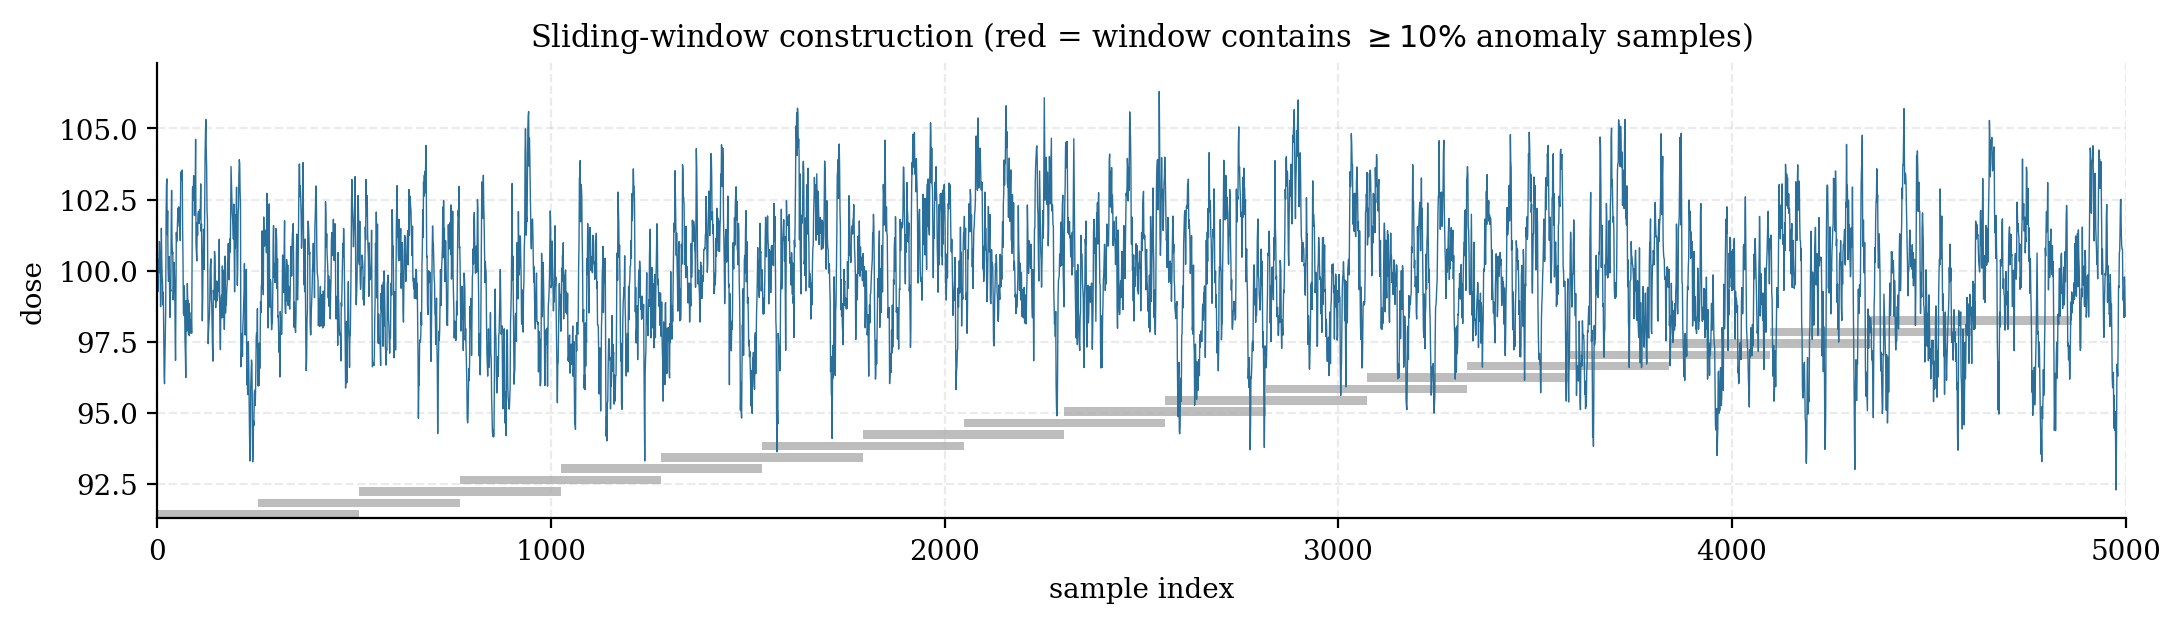
\includegraphics[width=0.92\linewidth]{sliding_window}
  \vspace{-0.2em}
  \begin{itemize}\footnotesize
    \item \textbf{Temporal split first} (first $80\%$ train$+$val, last $20\%$
          test), \emph{then} window $\Rightarrow$ no leakage between overlapping
          windows. $W=512$, stride $32$ at training.
    \item \textbf{Coverage labelling:} a window is anomalous (majority anomaly
          class) iff $\ge \tau_{\mathrm{cov}}=10\%$ of its samples fall inside an
          event; otherwise \texttt{Normal}.
    \item \textbf{Per-window normalisation:}
          $\tilde{\mathbf{x}}^{(t)} =
           \big(\mathbf{x}^{(t)} - \overline{\mathbf{x}^{(t)}}\big)/\sigma_{\mathrm{train}}$,
          with $\sigma_{\mathrm{train}}=4.21$ (a single global std, reused at
          inference). The network sees only deviations from the local baseline.
  \end{itemize}
\end{frame}

\begin{frame}{Building blocks --- convolution, normalisation, residual}
  \footnotesize
  \begin{block}{1D convolution}
    \vspace{-0.6em}
    \[
      \mathbf{v}_{c,t} = b_c + \sum_{c'=1}^{C_{\mathrm{in}}}\sum_{i=1}^{k}
        \mathbf{w}_{c,c',i}\;\mathbf{u}_{c',\,s\,t+i-p}.
    \]
    \vspace{-0.6em}\\
    $\mathbf{u}\in\R^{C_{\mathrm{in}}\times L}$ input ($C_{\mathrm{in}}$
    channels, length $L$); $\mathbf{w}\in\R^{C_{\mathrm{out}}\times
    C_{\mathrm{in}}\times k}$ kernel (width $k$); $s$ stride; $p$ padding; $b_c$
    bias; $\mathbf{v}$ output. Weight sharing $\Rightarrow$ translation
    equivariance; parameters $C_{\mathrm{out}}C_{\mathrm{in}}k$ \emph{independent
    of} $L$. Then $\ReLU(z)=\max(0,z)$, max-pooling, and
    \texttt{AdaptiveAvgPool1d(4)} (keeps $4$ temporal bins).
  \end{block}
  \begin{block}{Normalisation \quad/\quad Residual block}
    \textbf{BatchNorm} standardises each channel over the mini-batch (running
    stats differ train vs inference); \textbf{GroupNorm} standardises over
    channel \emph{groups per sample} --- identical at train/inference,
    amplitude-invariant. We use BN in the baseline, GroupNorm($8$) in the two
    deeper models.
    \[
      \mathrm{Res}(\mathbf{u}) = \ReLU\!\big(\mathbf{u} + \mathcal{F}(\mathbf{u})\big),
      \qquad \mathcal{F} = \Conv\!-\!\GN\!-\!\ReLU\!-\!\Conv\!-\!\GN,
    \]
    with a $1{\times}1$ conv on the shortcut when the channel count changes. The
    identity shortcut keeps deep stacks trainable (no vanishing gradient).
  \end{block}
\end{frame}

\begin{frame}{Building blocks --- self-attention}
  \begin{columns}[T]
    \begin{column}{0.62\linewidth}
      \footnotesize
      Token sequence $\mathbf{Z}\in\R^{T\times d}$: $T$ tokens (time steps),
      dimension $d$.
      \[
        \mathbf{Q}=\mathbf{Z}\mathbf{W}^{Q},\;
        \mathbf{K}=\mathbf{Z}\mathbf{W}^{K},\;
        \mathbf{V}=\mathbf{Z}\mathbf{W}^{V},
      \]
      \[
        \Attn(\mathbf{Q},\mathbf{K},\mathbf{V})
          = \softmax\!\Big(\tfrac{\mathbf{Q}\mathbf{K}^{\top}}{\sqrt{d_h}}\Big)\mathbf{V}.
      \]
      $\mathbf{W}^{Q},\mathbf{W}^{K},\mathbf{W}^{V}\in\R^{d\times d_h}$ learnable
      ($d_h$ = per-head dimension). Rows of $\softmax(\cdot)\in\R^{T\times T}$
      sum to $1$ $\Rightarrow$ each output is a \alert{convex combination of the
      value vectors} (learnt, content-based weighting).
      \begin{itemize}
        \item One attention layer lets \emph{every} position see the whole
              window (unlike a bounded convolution).
        \item $h$ heads in parallel (multi-head); a fixed \alert{sinusoidal
              positional encoding} is added (attention is order-agnostic); a
              learnable \texttt{[CLS]} token is read out for classification.
      \end{itemize}
    \end{column}
    \begin{column}{0.38\linewidth}
      \centering
      \resizebox{\linewidth}{!}{%
      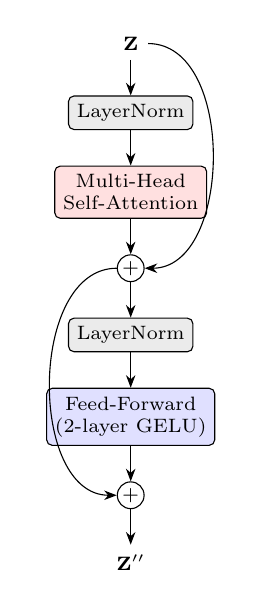
\begin{tikzpicture}[
          font=\scriptsize,
          block/.style={draw, rounded corners=2pt, align=center, minimum height=0.3cm, inner sep=3pt},
          attn/.style={block, fill=red!12},
          ffn/.style={block, fill=blue!12},
          norm/.style={block, fill=black!8},
          ar/.style={-{Stealth[length=1.6mm]}}, node distance=0.45cm]
        \node (in) {$\mathbf{Z}$};
        \node[norm, below=of in] (ln1) {LayerNorm};
        \node[attn, below=of ln1] (mha) {Multi-Head\\Self-Attention};
        \node[circle, draw, below=of mha, minimum size=3.4mm, inner sep=0pt] (add1) {$+$};
        \node[norm, below=of add1] (ln2) {LayerNorm};
        \node[ffn, below=of ln2] (ffn) {Feed-Forward\\(2-layer GELU)};
        \node[circle, draw, below=of ffn, minimum size=3.4mm, inner sep=0pt] (add2) {$+$};
        \node[below=of add2] (out) {$\mathbf{Z}''$};
        \draw[ar] (in)--(ln1); \draw[ar] (ln1)--(mha); \draw[ar] (mha)--(add1);
        \draw[ar] (add1)--(ln2); \draw[ar] (ln2)--(ffn); \draw[ar] (ffn)--(add2);
        \draw[ar] (add2)--(out);
        \draw[ar] (in.east) to[out=0,in=0] (add1.east);
        \draw[ar] (add1.west) to[out=180,in=180] (add2.west);
      \end{tikzpicture}}
      \\[0.3em]
      {\scriptsize Pre-LN Transformer encoder block (residual around each
       sub-layer).}
    \end{column}
  \end{columns}
\end{frame}

\begin{frame}{Three architectures of increasing complexity}
  Shared interface: input a single-channel window $\mathbf{x}\in\R^{1\times512}$,
  output $K=7$ logits.
  \begin{table}
    \centering\footnotesize
    \begin{tabular}{lccc}
      \toprule
      & \textbf{\dCNN} & \textbf{\dResNet} & \textbf{\dAttn} \\
      \midrule
      Trunk             & 3 plain conv blocks & 3 residual blocks & stride-2 stem $+$ 2 encoders \\
      Normalisation     & BatchNorm           & GroupNorm(8)      & GroupNorm(8) $+$ LayerNorm \\
      Long-range mixing & ---                 & ---               & multi-head self-attention \\
      Parameters        & $22{,}727$          & $74{,}631$        & $109{,}655$ \\
      \bottomrule
    \end{tabular}
  \end{table}
  \footnotesize
  \begin{itemize}
    \item \textbf{A --- \dCNN{} (baseline):} 3 $\times$
          Conv--BN--ReLU--MaxPool (kernels $7,7,5$; channels
          $16\!\to\!32\!\to\!64$) $+$ MLP head. Sanity check on the pipeline.
    \item \textbf{B --- \dResNet:} same depth, each block residual with
          GroupNorm; \emph{identical head} $\Rightarrow$ a clean ablation of the
          residual trunk.
    \item \textbf{C --- \dAttn:} stride-2 conv stem $\to T=64$ tokens of
          dimension $d=64$, then $2$ pre-norm Transformer encoders ($h=4$ heads);
          \texttt{[CLS]} output feeds a linear classifier.
  \end{itemize}
\end{frame}

% =============================================================================
\section{Results}
% =============================================================================

\begin{frame}{Training dynamics and window-level accuracy}
  \begin{columns}[T]
    \begin{column}{0.62\linewidth}
      \centering
      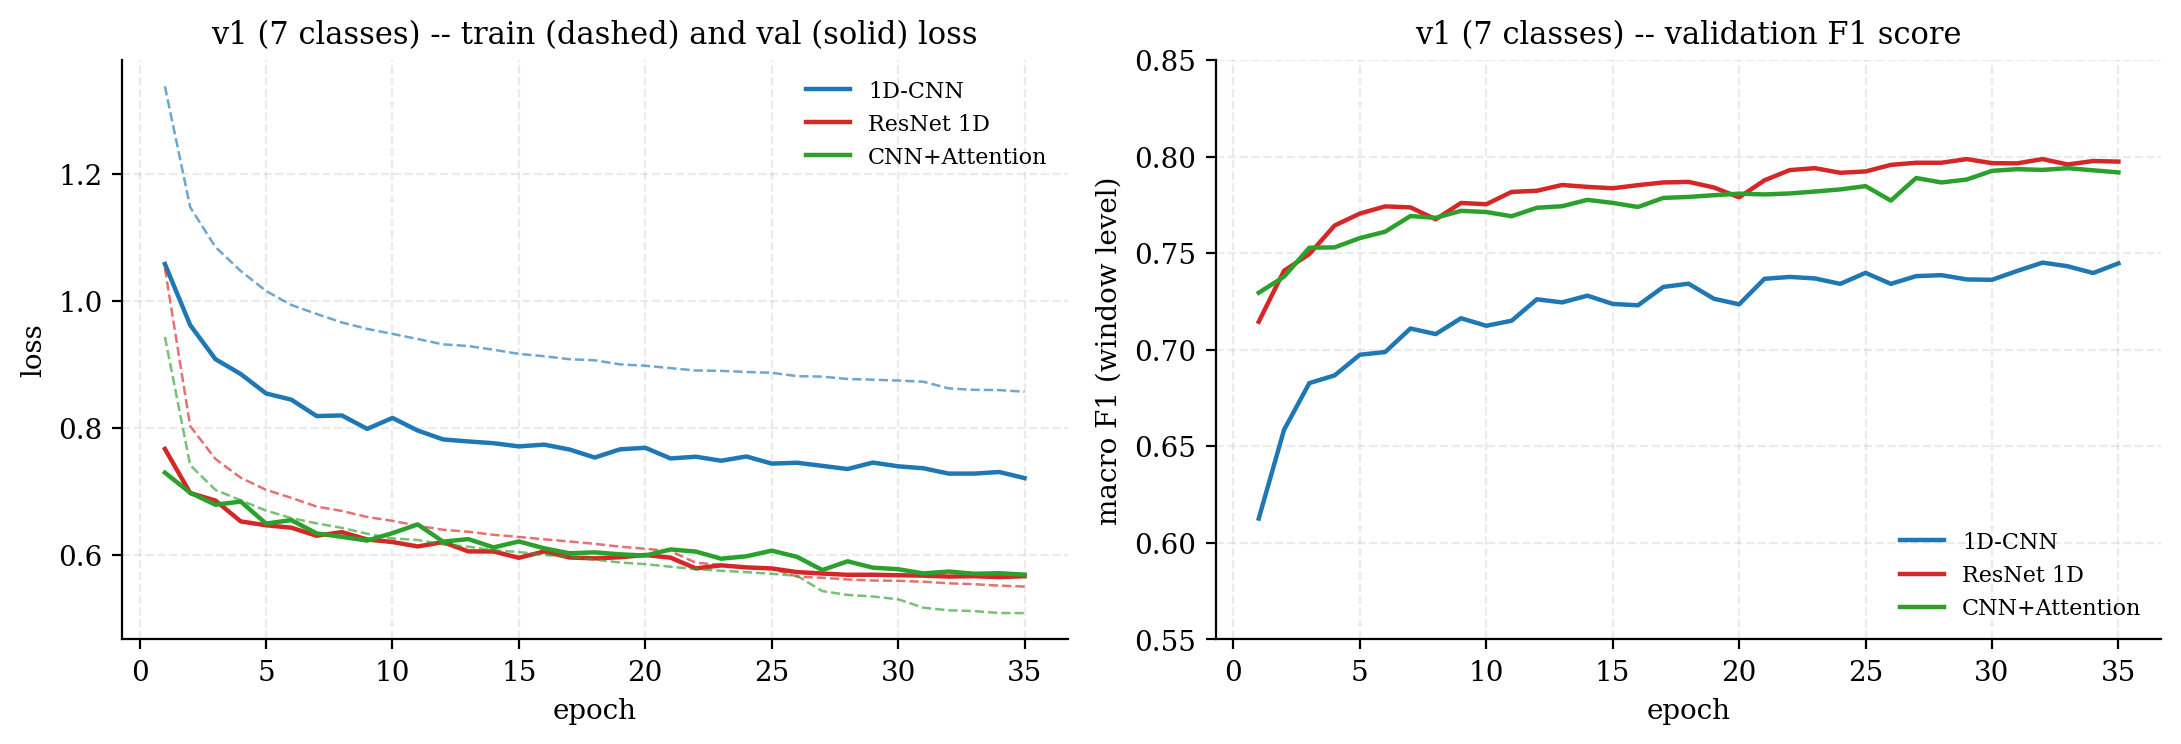
\includegraphics[width=\linewidth]{v1_training_curves}\\[0.2em]
      {\scriptsize Train/val loss (left) and validation macro $F_1$ (right).}
    \end{column}
    \begin{column}{0.38\linewidth}
      \footnotesize
      \begin{itemize}
        \item All converge within $35$ epochs.
        \item The two deeper models reach a lower val loss ($\approx0.57$ vs
              $\approx0.72$) and a higher val $F_1$.
      \end{itemize}
      \begin{table}
        \centering\scriptsize
        \begin{tabular}{lc}
          \toprule
          Overall window acc. & \\
          \midrule
          \dCNN        & $0.766$ \\
          \dResNet     & $\mathbf{0.807}$ \\
          \dAttn       & $0.795$ \\
          \bottomrule
        \end{tabular}
      \end{table}
      {\scriptsize Background $\sim\!94\%$ for all; \texttt{bell\_sq} is the
       hardest (a \texttt{bell} with a plateau). Depth helps.}
    \end{column}
  \end{columns}
\end{frame}

\begin{frame}{Event-level evaluation (59-event synthetic segment)}
  \centering
  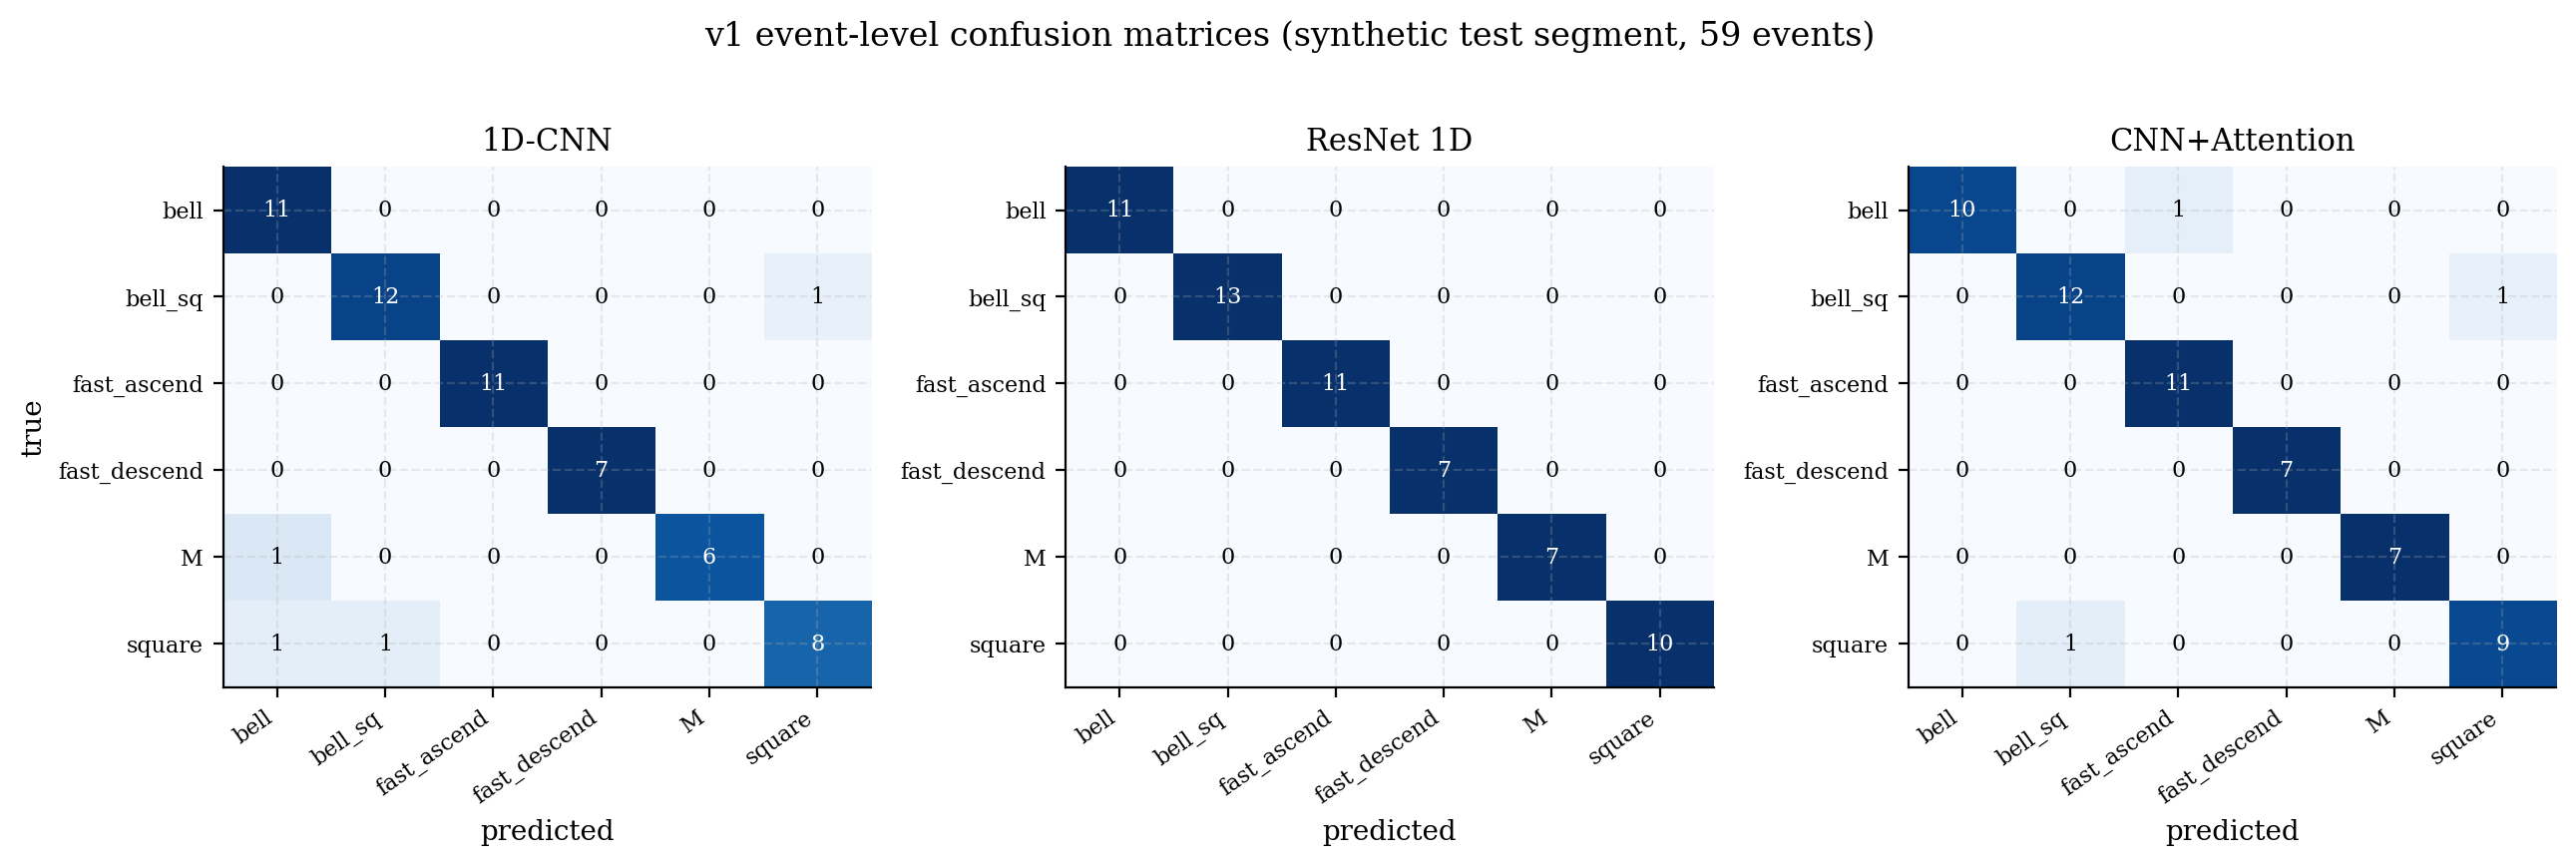
\includegraphics[width=0.97\linewidth]{v1_confusion_matrices}
  \begin{columns}[T]
    \begin{column}{0.52\linewidth}
      \begin{table}
        \centering\scriptsize
        \begin{tabular}{lcccc}
          \toprule
          Model & Hits & Miss & FA & Macro $F_1$ \\
          \midrule
          \dCNN        & 55 & 4 & 0 & $0.934$ \\
          \dResNet     & 59 & 0 & 0 & $\mathbf{1.000}$ \\
          \dAttn       & 56 & 3 & 0 & $0.955$ \\
          \bottomrule
        \end{tabular}
      \end{table}
    \end{column}
    \begin{column}{0.48\linewidth}
      \footnotesize
      \begin{itemize}
        \item Events matched by interval overlap (FA = false alarm).
        \item \alert{No false alarms} on the segment; the \dResNet{} classifies
              \alert{all 59 events}; the other two miss visually similar
              morphologies.
      \end{itemize}
    \end{column}
  \end{columns}
\end{frame}

\begin{frame}{Robustness to distribution shift}
  \centering
  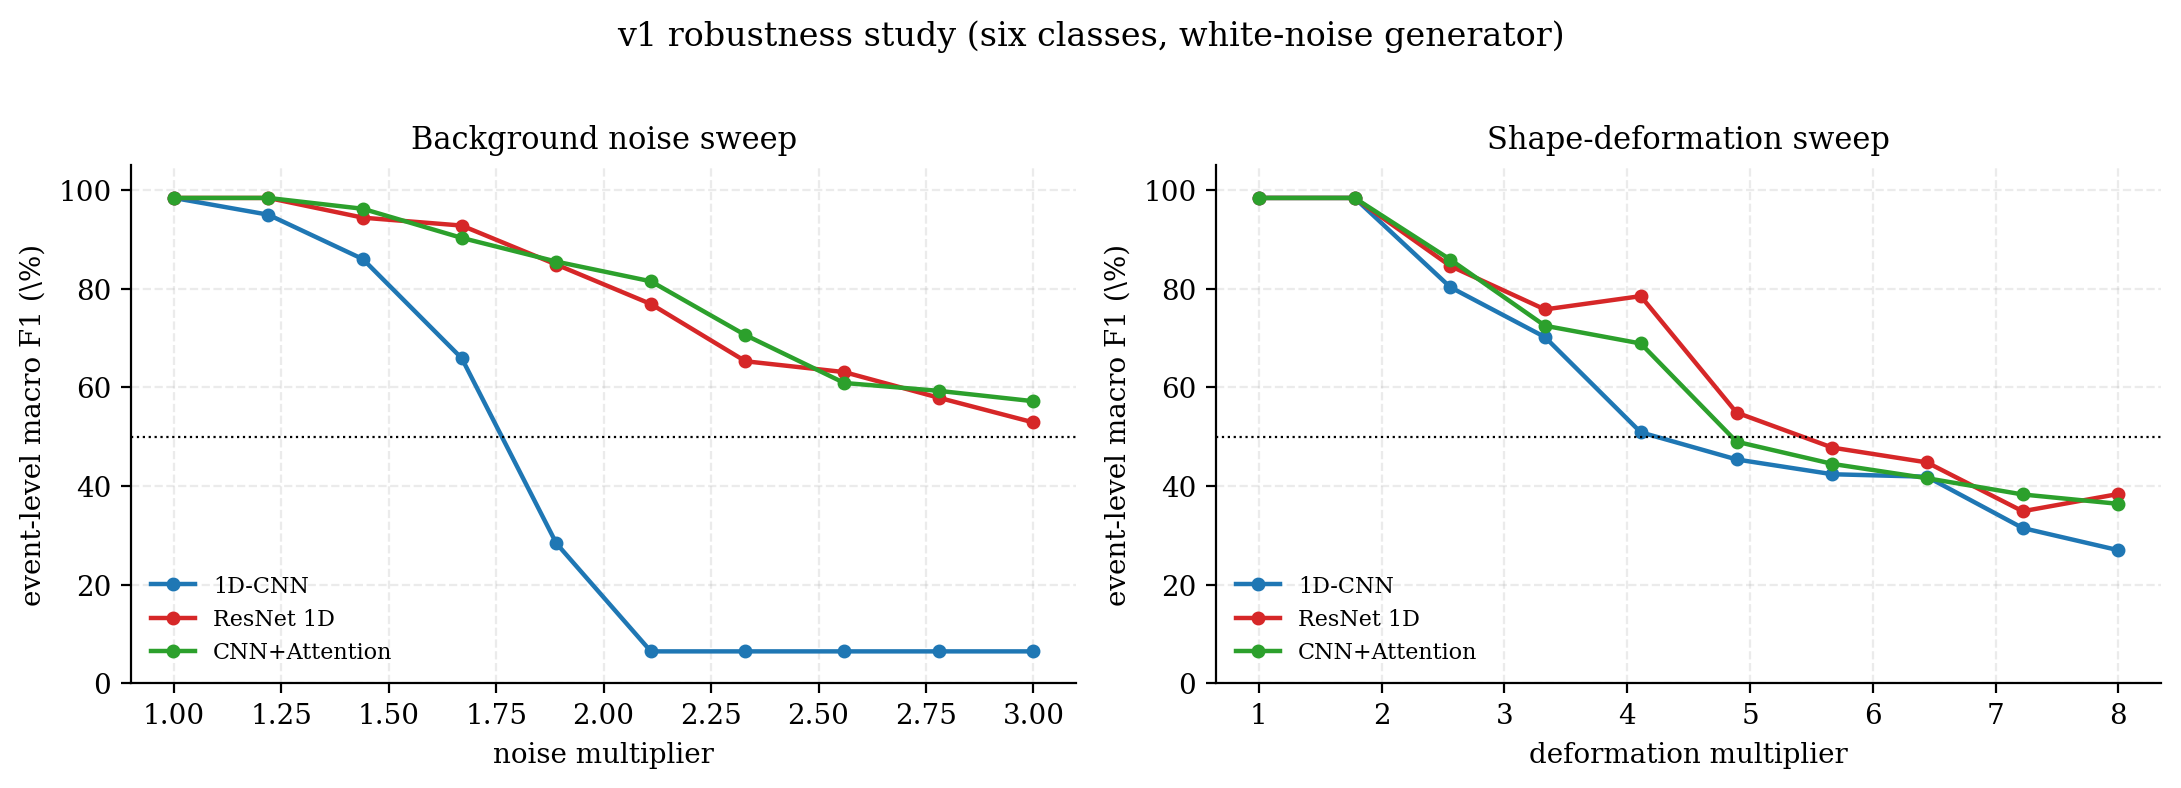
\includegraphics[width=0.93\linewidth]{v1_robustness}
  \begin{itemize}\footnotesize
    \item Two axes (small regenerated test sets): background-noise multiplier
          $m_{\mathrm{noise}}\in[1,3]$ (noise \emph{texture}, amplitude scaled
          with it) and shape-deformation multiplier $m_{\mathrm{deform}}\in[1,8]$.
          All start near $98\%$.
    \item \textbf{Noise:} the \dCNN{} drops below $50\%$ by
          $m_{\mathrm{noise}}\!\approx\!1.9$ then \alert{collapses to a single
          class ($\sim 6\%$)}; \dResNet{} \& \dAttn{} stay $\ge 53$--$57\%$ to
          $3\times$. \textbf{Deformation:} all degrade gracefully ($<50\%$ at
          $4.9$ / $5.7$ / $4.9$).
    \item \alert{GroupNorm $+$ residual} buy the noise robustness; the baseline's
          batch-norm running statistics become invalid under the shift.
  \end{itemize}
\end{frame}

\begin{frame}{Computational cost and discussion}
  \begin{table}
    \centering\footnotesize
    \begin{tabular}{lcccc}
      \toprule
      Model & Parameters & Train time & Inference (win/s) & Event $F_1$ \\
      \midrule
      \dCNN        & $22{,}727$  & $\sim 4.3$ min & $\sim 10{,}700$ & $0.934$ \\
      \dResNet     & $74{,}631$  & $\sim 10.0$ min & $\sim 14{,}200$ & $\mathbf{1.000}$ \\
      \dAttn       & $109{,}655$ & $\sim 10.2$ min & $\sim 15{,}200$ & $0.955$ \\
      \bottomrule
    \end{tabular}
    \caption*{\scriptsize Single RTX 5060 Laptop GPU.}
  \end{table}
  \begin{itemize}\footnotesize
    \item \textbf{Residual learning $+$ GroupNorm is the biggest win}: at equal
          depth and identical head, \dResNet{} beats the plain \dCNN{} on every
          axis, and the gap explodes under noise.
    \item \textbf{Self-attention buys no extra robustness here}: $W=512$ with
          events $\le 800$ samples leaves little long-range context for attention
          to exploit.
    \item \textbf{The cheapest model is the most fragile}: the \dCNN's
          single-class collapse makes it unsuitable across seasons.
    \item $\Rightarrow$ \alert{\dResNet{} 1D is the best trade-off} of accuracy,
          robustness and cost.
  \end{itemize}
\end{frame}

% =============================================================================
\section{Conclusion and perspectives}
% =============================================================================

\begin{frame}{Conclusion and recommendation}
  \begin{itemize}
    \item Formalised radiological-event identification as \alert{sliding-window
          multi-class classification} of a noisy gamma-dose signal, and validated
          a deep-learning approach on a controlled, calibrated synthetic
          benchmark.
    \item All three architectures reach strong event-level performance (macro
          $F_1$ from $0.93$ to $1.00$, no false alarms).
    \item The \dResNet{} is best overall --- perfect event score, highest window
          accuracy, and (with the hybrid) the only model that resists
          background-noise growth, while the baseline collapses. Attention did
          \emph{not} help at the $512$-sample window scale.
  \end{itemize}
  \begin{block}{Recommendation}
    \textbf{\dResNet{} 1D} --- best accuracy and robustness at moderate cost
    ($\sim 75$k params, $\sim 10$ min on a laptop GPU). The \dCNN{} only if
    compute is very constrained \emph{and} noise is stable; the \dAttn{} if
    windows are later extended to capture long-range context.
  \end{block}
\end{frame}

\begin{frame}{Limitations and perspectives}
  \begin{columns}[T]
    \begin{column}{0.5\linewidth}
      \textbf{Limitations}
      \begin{itemize}\footnotesize
        \item Results are, by construction, \alert{synthetic}.
        \item HF noise is independent in time (real sensor noise is correlated).
        \item Anomaly density far higher than a real beacon's.
        \item No labelled real test set $\Rightarrow$ real performance not yet
              measurable.
      \end{itemize}
    \end{column}
    \begin{column}{0.5\linewidth}
      \textbf{Perspectives --- ``to go further''}
      \begin{itemize}\footnotesize
        \item \alert{Realistic signal models}: coloured (autoregressive) noise
              matching the real autocorrelation; lower density; calibrated
              morphologies --- \emph{same pipeline} re-run.
        \item \alert{A labelled real test set}: first real event-level precision
              / recall.
        \item \alert{Explainability}: Grad-CAM on conv feature maps; attention
              maps.
        \item \alert{Longer windows \& richer inputs}: meteorological channels;
              the context attention lacked here.
      \end{itemize}
    \end{column}
  \end{columns}
\end{frame}

% ── Closing ──────────────────────────────────────────────────────────────────
\begin{frame}[standout]
  Thank you --- questions?
  \vspace{0.6em}\\
  {\normalsize\normalfont On a clean, controlled benchmark the approach works;
   \emph{depth and group normalisation}, not attention, buy robustness at this
   window length.}
\end{frame}

% =============================================================================
\appendix
% =============================================================================

\begin{frame}{Backup --- shared training / inference settings}
  \begin{table}
    \centering\footnotesize
    \begin{tabular}{ll}
      \toprule
      Setting & Value \\
      \midrule
      Window $W$ / stride (train / inf.)     & $512$ \;/\; $32$ \;/\; $10$ \\
      Labelling threshold $\tau_{\mathrm{cov}}$ & $0.10$ (majority anomaly class) \\
      Normalisation                          & per-window centring, $\sigma_{\mathrm{train}}=4.21$ \\
      Split                                  & temporal $80/20$, then random $80/20$ on train \\
      Optimiser                              & Adam ($\beta_1{=}0.9,\beta_2{=}0.999,\varepsilon{=}10^{-8}$) \\
      Learning rate / batch                  & $10^{-3}$ / $128$, max $35$ epochs \\
      LR scheduler / early stopping          & \texttt{ReduceLROnPlateau}(2, $0.5$) / patience $10$ \\
      Loss / class weights $\mathbf{w}$      & weighted CE; $(0.46,1.18,1.27,1.32,1.24,1.15,1.31)$ \\
      Train / test windows                   & $249{,}985$ / $62{,}485$ \\
      Event extraction                       & bg-prob.\ threshold $0.3$, bridge gaps $\le 50$ \\
      \bottomrule
    \end{tabular}
  \end{table}
\end{frame}

\begin{frame}{Backup --- synthetic generator configuration}
  \begin{table}
    \centering\footnotesize
    \begin{tabular}{ll}
      \toprule
      Parameter & Value \\
      \midrule
      Total length $N$        & $10^{7}$ samples (written in $5\cdot10^{4}$ chunks) \\
      Number of anomalies     & $5{,}000$--$8{,}000$ ($\sim 6$--$8$ / $10$k samples) \\
      Injection jitter        & $\pm 200$ samples \\
      Anomaly amplitude       & $\sigma\cdot\mathcal{U}(2.5,7.6)$ (SNR units) \\
      Anomaly duration        & $\mathcal{U}[200,800]$ samples \\
      Deformation level $\nu$ & $\mathcal{U}(0.02,0.10)$ \\
      HF noise                & i.i.d.\ $\mathcal{N}(0,\sigma^2)$, $\sigma=2.53$ \\
      Baseline (OU)           & $\mu=99.26,\ \theta=4\cdot10^{-6},\ \sigma_{\mathrm{OU}}=0.0373$ \\
      Templates / classes     & 6 morphologies $+$ background ($K=7$) \\
      \bottomrule
    \end{tabular}
  \end{table}
\end{frame}

\begin{frame}[allowframebreaks]{Backup --- key references}
  \footnotesize
  \begin{thebibliography}{99}
    \setbeamertemplate{bibliography item}[text]
    \bibitem{fawaz} H.\ Ismail Fawaz et al. \emph{Deep learning for time series
      classification: a review.} DMKD, 2019.
    \bibitem{wang} Z.\ Wang, W.\ Yan, T.\ Oates. \emph{Time series classification
      from scratch with deep neural networks: a strong baseline.} IJCNN, 2017.
    \bibitem{bai} S.\ Bai, J.\ Z.\ Kolter, V.\ Koltun. \emph{An empirical
      evaluation of generic convolutional and recurrent networks for sequence
      modeling.} arXiv:1803.01271, 2018.
    \bibitem{lecun} Y.\ LeCun et al. \emph{Gradient-based learning applied to
      document recognition.} Proc.\ IEEE, 1998.
    \bibitem{he} K.\ He, X.\ Zhang, S.\ Ren, J.\ Sun. \emph{Deep residual
      learning for image recognition.} CVPR, 2016.
    \bibitem{ioffe} S.\ Ioffe, C.\ Szegedy. \emph{Batch normalization.} ICML, 2015.
    \bibitem{wu} Y.\ Wu, K.\ He. \emph{Group normalization.} ECCV, 2018.
    \bibitem{ba} J.\ L.\ Ba, J.\ R.\ Kiros, G.\ E.\ Hinton. \emph{Layer
      normalization.} arXiv:1607.06450, 2016.
    \bibitem{vaswani} A.\ Vaswani et al. \emph{Attention is all you need.}
      NeurIPS, 2017.
    \bibitem{devlin} J.\ Devlin et al. \emph{BERT: pre-training of deep
      bidirectional transformers.} NAACL-HLT, 2019.
    \bibitem{hu} Z.\ Hu, L.\ Chen. \emph{EEG-based emotion recognition using a
      CNN with multi-head self-attention.} Applied Sciences, 2022.
    \bibitem{blazquez} A.\ Bl\'azquez-Garc\'ia et al. \emph{A review on
      outlier/anomaly detection in time series data.} ACM CSUR, 2021.
    \bibitem{kingma} D.\ P.\ Kingma, J.\ Ba. \emph{Adam: a method for stochastic
      optimization.} ICLR, 2015.
    \bibitem{selvaraju} R.\ R.\ Selvaraju et al. \emph{Grad-CAM: visual
      explanations from deep networks.} ICCV, 2017.
    \bibitem{paszke} A.\ Paszke et al. \emph{PyTorch.} NeurIPS, 2019.
  \end{thebibliography}
\end{frame}

\end{document}
